


\documentclass[11pt]{article}

\usepackage[utf8]{inputenc} 
\usepackage[T1]{fontenc} 
\usepackage{graphicx}
\usepackage{grffile}
\usepackage{mathpazo} 
\usepackage{indentfirst}
\usepackage[section]{placeins}
\usepackage{url}
\usepackage{hyperref}

\begin{document}



%----------------------------------------------------------------------------------------
%	TITLE PAGE
%----------------------------------------------------------------------------------------

\begin{titlepage}
	\newcommand{\HRule}{\rule{\linewidth}{0.5mm}} 
	
	\center
	
	%------------------------------------------------
	%	Headings
	%------------------------------------------------
	
	\textsc{\LARGE Université Paris Dauphine}\\[1.5cm] 
	
	\textsc{\Large Master 1 MIAGE}\\[0.5cm] 
	

	
	%------------------------------------------------
	%	Title
	%------------------------------------------------
	
	\HRule\\[0.4cm]
	
	{\huge\bfseries Projet d'Intelligence Artificielle}\\[0.4cm]
	
	\HRule\\[1.5cm]
	
	%------------------------------------------------
	%	Author(s)
	%------------------------------------------------
	
	\begin{minipage}{0.4\textwidth}
		\begin{flushleft}
			\large
			\textit{Réalisé par :}\\
			Lyes \textsc{MEGHARA}\\ 
			Nadia \textsc{MSELLEK}\\ 
		\end{flushleft}
	\end{minipage}
	~
	\begin{minipage}{0.4\textwidth}
		\begin{flushright}
			\large
			\textit{Encadré par :}\\
			Mr Stephane \textsc{AIRIAU}% Supervisor's name

		\end{flushright}
	\end{minipage}
	

	
	
	\vfill\vfill 
	
	{\large18 Décembre 2017} 
	



	\leavevmode \newline 	\leavevmode \newline 	\leavevmode \newline 	\leavevmode \newline 	\leavevmode \newline 
	
\includegraphics[width=0.6\textwidth]{dauphine.png}\\[1cm] 
	 

	

	
\end{titlepage}

\renewcommand{\thesection}{\Roman{section}}
\renewcommand{\thesubsection}{\thesection.\Roman{subsection}}





\section{Introduction}


La notion de réseaux de neurones artificiels a été évoquée depuis plus de cinquante ans. Cela a permis l’évolution concrète de l’intelligence artificielle au plus grand bonheur des informaticiens et étudiants. Le projet que nous allons exposer traite de la capacité d’un algorithme d’apprentissage supervisé suivant le modèle du perceptron. \newline  \newline
Nous disposons pour cela d’une base de données créée par Yann \textsc{LECUN} nommée « \textit {Mnist handwritten database} » composée de plusieurs milliers d’exemples d’images de 28*28 pixels chacune représentant un chiffre manuscrit. \newline
Notre objectif est de récupérer parmi cette base de données un fichier input contenant 60 000 exemples sur lesquels notre algorithme va « apprendre » et ainsi pouvoir prédire les chiffres contenus sur chacun des 10 000 exemples donnés pour le test.\newline 



\section{Outils de développement}

Dans le cadre de ce projet, nous avons utilisé GitHub pour une meilleure collaboration, eclipse sous la JDK 1.8, Doxygène nous a permis de générer une documentation visible depuis le fichier index.html. \newline Pour finir ce rapport a été rédigé en utilisant LateX.



\section{Résultats des tests}

Avec un SingleLayer, l'exécution pour 28*28 neurones d'entrées ainsi que 10 neurones de sorties dure 5 minutes, cette dernière corrige lentement le taux d'erreurs et avoisine les 8\%
 à la fin de l'exécution. \newline

Un HiddenLayer, cette fois-ci, avec 10 neurones cachés donne à priori les mêmes résultats pour le même temps d'exécutions, en revanche, en passant à 20 neurones cachés, les courbes se croisent, celle du réseau caché passe en dessous comme visible à la figure 2, augmenter le nombre des neurones cachés améliore l'apprentissage, mais ralentit fortement l'exécution.\newline

\begin{figure}[!htb]
  \centering
    \caption{Résultat d'entrainement d'un SingleLayer}
    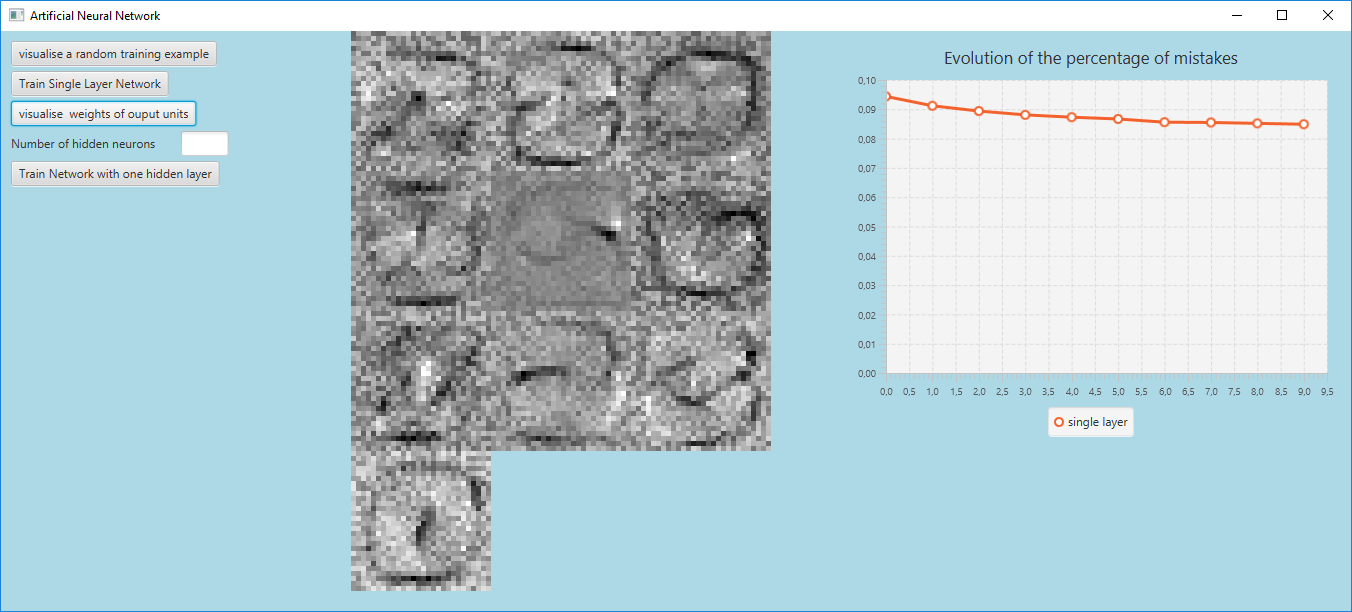
\includegraphics[width=\textwidth]{single.png}
	\textit {The training of your single layer lasted for 310.314633146 seconds}
\newline \newline

  \centering
    \caption{Résultat d'entrainement d'un HiddenLayer}
    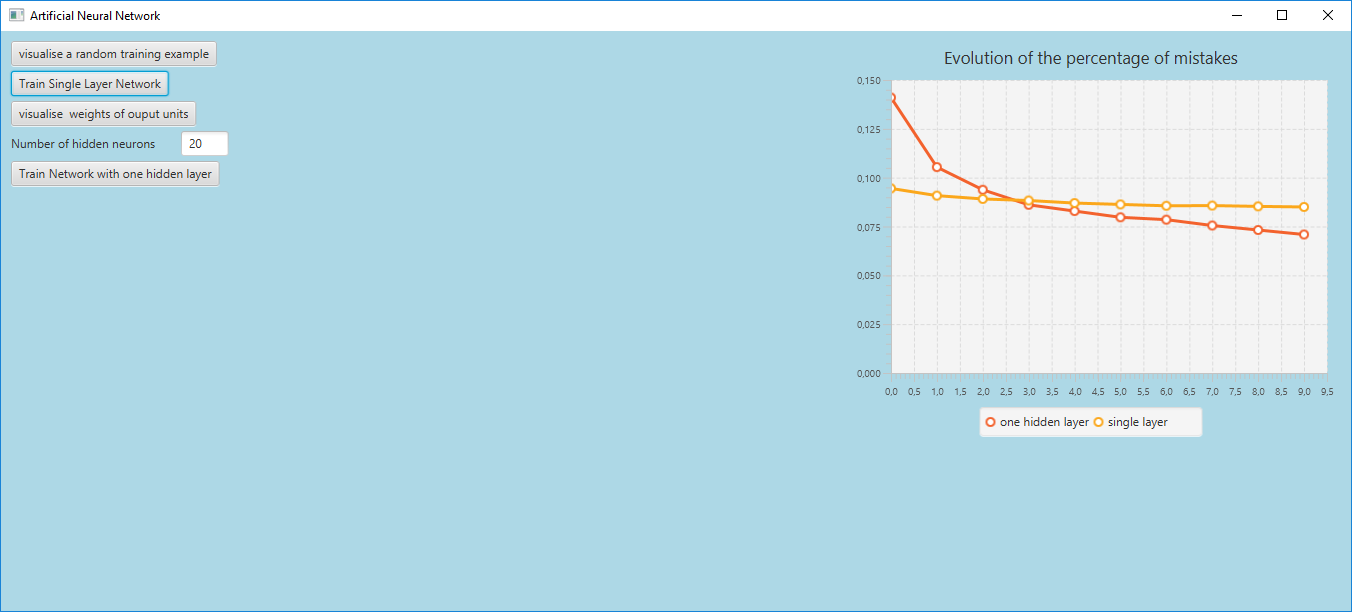
\includegraphics[width=\textwidth]{hidden.png}
	\textit {The training of your hidden layer lasted for 662.522861786 seconds}

\end{figure}




\section{Conclusion sur les résultats}

Comme nous aurions pu le prédire, les résultats de HiddenLayer nous fournissent beaucoup moins d’erreurs que SingleLayer. Nous pouvions en effet conjecturer que, puisque HiddenLayer pouvait avoir beaucoup plus de neurones que SingleLayer, il aurait plus de \textit{synapses}; si l’on veut faire l’analogie avec le cerveau humain; et donc plus de variables à modifier, donc un apprentissage plus efficace. \newline
Néanmoins, il est important de souligner que le SingeLayer lors de ses débuts, apprend bien mieux que le HiddenLayer, sur la durée, HiddenLayer le rattrape et le dépasse . \newline
Ici, une seule couche cachée permet déjà d’atteindre un degré d’erreur assez faible. On suppose, naturellement, que de meilleurs résultats peuvent être atteints avec plusieurs couches cachées. 

D'autre part, augmenter le nombre d'itérations à 20, ne permet pas d'avoir une amélioration significative, en effet au bout de la 15eme itération, notre algorithme n'apprend plus, et reste à un nombre d'erreurs quasi constant. En revanche, augmenter le nombre de neurones cachés à 80, améliore significativement les résultats et aboutit à 5\% d'erreurs au détriment d'un temps d'exécution très lent.





\section{Ressenti de l'implémentation}

Il est important de souligner que mis à part le cours, avant de travailler sur ce projet nous n’avions pas d’expérience avec les réseaux de neurones artificiels. \newline
En outre, la première difficulté a été de comprendre le code déjà existant, les différentes classes et le lien entre ces dernières, comme les méthodes s'appellent et sont liées entre elles, trouver la source de nos erreurs n'a pas toujours été une tâche aisée.  \newline 
Une des principales difficultés relevées a été l’implémentation de la méthode train pour la classe SingleLayer, qui affichait une courbe constante avant correction de notre part. Le passage de SingleLayer à HiddenLayer a été plus fluide de sens et de logique. \newline

\section{Améliorations éventuelles / Hypothèses }

Le programme étant assez lent à tourner, une des premières idées que nous avons eues, était d'accroitre sa vitesse, en passant par des Threads, solution qui n'a pas été implémentée par manque de temps. \newline 
D'autres points, sur le côté théorique cette fois-ci, l'utilisation de biais n'a pas été mentionnée de façon explicite dans ce cours.  \newline
Par ailleurs, l'algorithme d'apprentissage \textit {Widrow-Hoff} a été préféré à \textit {l'algorithme de gradient}, étant à la fois plus efficace, et plus simple à implémenter. 

\clearpage

\section{Webographie} 
\begin{itemize}
\item \url{https://fr.wikipedia.org/wiki/Perceptron} \newline
\item \url{https://fr.wikipedia.org/wiki/Perceptron_multicouche} \newline
\item \url{alp.developpez.com/tutoriels/intelligence-artificielle/reseaux-de-neurones/} \newline
\item \url{https://towardsdatascience.com/multi-layer-neural-networks-with-sigmoid-function-deep-learning-for-rookies-2-bf464f09eb7f} \newline
\item \url{https://www.cs.cmu.edu/afs/cs/academic/class/15883-f15/slides/backprop.pdf} \newline
\item \url{http://www.dgp.toronto.edu/people/RMB/papers_old/p6.pdf} \newline
\item \url{https://www.labri.fr/perso/nrougier/downloads/Perceptron.pdf} \newline
\item \url{ http://www.turingfinance.com/misconceptions-about-neural-networks/} \newline
\item \url{https://youtu.be/L7WNYvbvGBc} \newline
\end{itemize}

\section{Annexes } 
 \begin{center}
    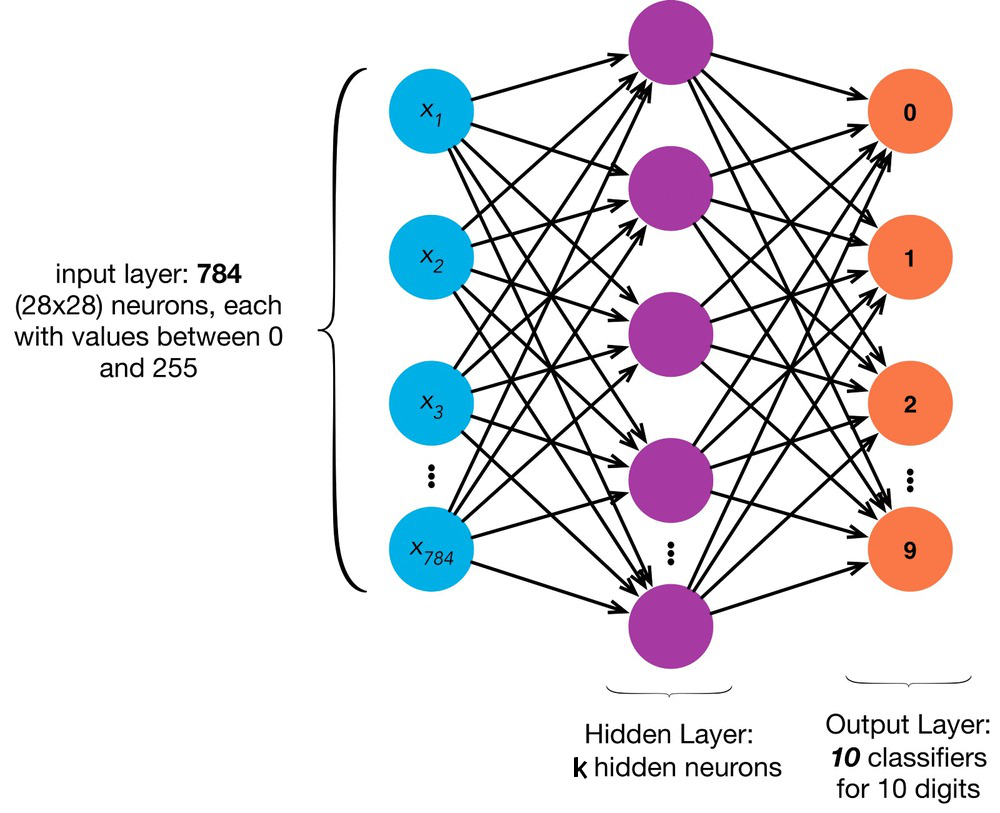
\includegraphics[width=\textwidth]{annexes.png}
\end{center}

\end{document}
